% ========== 第五章：实现细节 ==========
\chapter{实现细节}

本章在前两章方法设计与数据管线的基础上，给出训练流程、显存优化、收敛验证、推理应用与 ComfyUI 部署的具体实现细节。

\section{训练流程}

\subsection{模型加载与 LoRA 挂载}

训练脚本 \texttt{train\_lora.py} 首先从 HuggingFace Hub（或本地缓存）加载 InstructPix2Pix 的四个子模块：CLIPTokenizer、CLIPTextModel、AutoencoderKL、UNet2DConditionModel 和 DDPMScheduler。加载后立即验证 UNet conv\_in 的输入通道数为 8（断言保护），确保底模正确。

随后冻结所有底模参数（VAE、Text Encoder、UNet 原始权重），在 UNet 的注意力层上挂载 LoRA 适配器。LoRA 配置为：目标模块 \texttt{[to\_q, to\_k, to\_v, to\_out.0]}，秩 $r = 4$，$\alpha = r$，以高斯分布初始化。RotationEncoder 为随机初始化（或从断点恢复）的两层 MLP（$6 \to 256 \to 768$，SiLU 激活）。

\subsection{数据集与 DataLoader}

训练数据集 \texttt{AdjacentPairDataset}（\texttt{dataset.py}）从 \texttt{train\_manifest.json} 中加载所有场景的视角标注，按 elevation 分组后构建相邻视角对。每个样本返回：参考条件图张量（$3 \times 512 \times 512$，归一化至 $[-1, 1]$）、目标条件图张量（同尺寸）、相对旋转向量（$[\Delta\text{az}, \Delta\text{el}, \Delta\text{roll}]$，单位度）、以及物品名称 prompt 字符串。

DataLoader 采用 batch\_size = 1（受限于 16G 显存），shuffle = True。Windows 下为避免多进程 spawn 带来的重型依赖重复导入开销，默认 num\_workers = 0（主进程内加载）。

\subsection{训练循环}

训练使用 HuggingFace Accelerate 库管理混合精度与梯度累积。每个训练步：

\begin{enumerate}[label=(\arabic*)]
    \item 参考条件图与目标条件图分别经 VAE 编码为 latent $\mathbf{z}_c^{\text{ref}}$ 与 $\mathbf{z}_c^{\text{tgt}}$。
    \item 向 $\mathbf{z}_c^{\text{tgt}}$ 添加随机噪声得到 $\mathbf{z}_t$。
    \item 物品名称 prompt 经 CLIP tokenizer + text\_encoder 编码为 $(1, 77, 768)$ 文本嵌入。
    \item 旋转向量经 RotationEncoder 编码为 $(1, 1, 768)$ 旋转嵌入，与文本嵌入拼接为 $(1, 78, 768)$。
    \item $\mathbf{z}_t$ 与 $\mathbf{z}_c^{\text{ref}}$ 在通道维拼接为 8 通道输入，送入 UNet 预测噪声 $\hat{\boldsymbol{\epsilon}}$。
    \item 计算 $\mathcal{L}_{\text{MSE}} = \|\boldsymbol{\epsilon} - \hat{\boldsymbol{\epsilon}}\|_2^2$，执行反向传播。
    \item 每 \texttt{gradient\_accumulation\_steps} 步后更新一次优化器参数。
\end{enumerate}

优化器为 AdamW，初始学习率 $1 \times 10^{-4}$。每个 epoch 结束后将完整训练状态（LoRA adapter、RotationEncoder、优化器、epoch、global\_step）保存为 checkpoint，并支持从中断处恢复续训。

\section{显存优化}

面向 RTX 4060 16G 显存的硬件约束，训练流程集成了三项显存优化措施：

\begin{itemize}
    \item \textbf{混合精度训练}：默认 fp16，将模型前向/反向传播中的浮点运算降至半精度，显著降低显存占用与计算时间。
    \item \textbf{梯度检查点（Gradient Checkpointing）}：在 UNet 前向传播中不保存中间激活值，反向传播时重新计算，以时间换空间。
    \item \textbf{梯度累积}：batch\_size = 1 + gradient\_accumulation\_steps = 4，等效 batch size 为 4。每次仅前向单个样本，累积 4 步梯度后再统一更新参数，避免大 batch 带来的显存峰值。
\end{itemize}

上述配置下，训练全流程（模型权重 + 优化器状态 + LoRA 梯度 + 激活值）可稳定运行于 16G 显存，无需 CPU offload。

\section{收敛验证}

\texttt{verify\_lora\_convergence.py} 提供了一套不依赖 GPU 的自动化收敛判定脚本。训练过程中每 10 步记录一次 loss 到 \texttt{loss\_history.json}。收敛判定的三个维度：

\begin{enumerate}[label=(\arabic*)]
    \item \textbf{趋势下降}：将 loss 序列均分为前、中、后三段，要求后段均值较前段均值下降幅度 $\geq 15\%$（\texttt{min\_drop\_ratio}）。
    \item \textbf{稳定性}：取最后 20\% 的 loss 窗口，要求其标准差/均值比 $\leq 0.5$（\texttt{max\_tail\_std\_ratio}），判断是否收敛至稳定区间。
    \item \textbf{数值有效性}：检测 NaN/Inf，作为梯度爆炸的预警信号。
\end{enumerate}

三个条件同时满足时判定为"收敛通过"，脚本输出每个 LoRA 分支的详细信息与整体摘要。

\section{推理应用}

\subsection{Gradio 交互界面}

\texttt{inference\_app.py} 使用 Gradio 框架提供了一个完整的 Web 推理调试界面（图~\ref{fig:gradio_ui}）。界面功能包括：

\begin{itemize}
    \item \textbf{自动条件图提取}：用户上传参考 RGB 图后，系统即时调用 Depth Anything V2 与 Canny 算法分别提取深度图与轮廓图预览，无需等待点击生成按钮。
    \item \textbf{双分支独立推理}：depth 分支与 canny 分支各自加载独立的 LoRA checkpoint（或留空退化为 InstructPix2Pix 原生图生图模式），并行生成结果。
    \item \textbf{多步迭代可视化}：生成过程中保存每步中间结果，以 Gallery 形式展示完整的迭代轨迹。
    \item \textbf{参数可调}：支持调节旋转角度（azimuth $[-180^\circ, 180^\circ]$，elevation $[-90^\circ, 90^\circ]$）、单步步长、采样步数、guidance scale、随机种子等参数。
\end{itemize}

\begin{figure}[H]
    \centering
    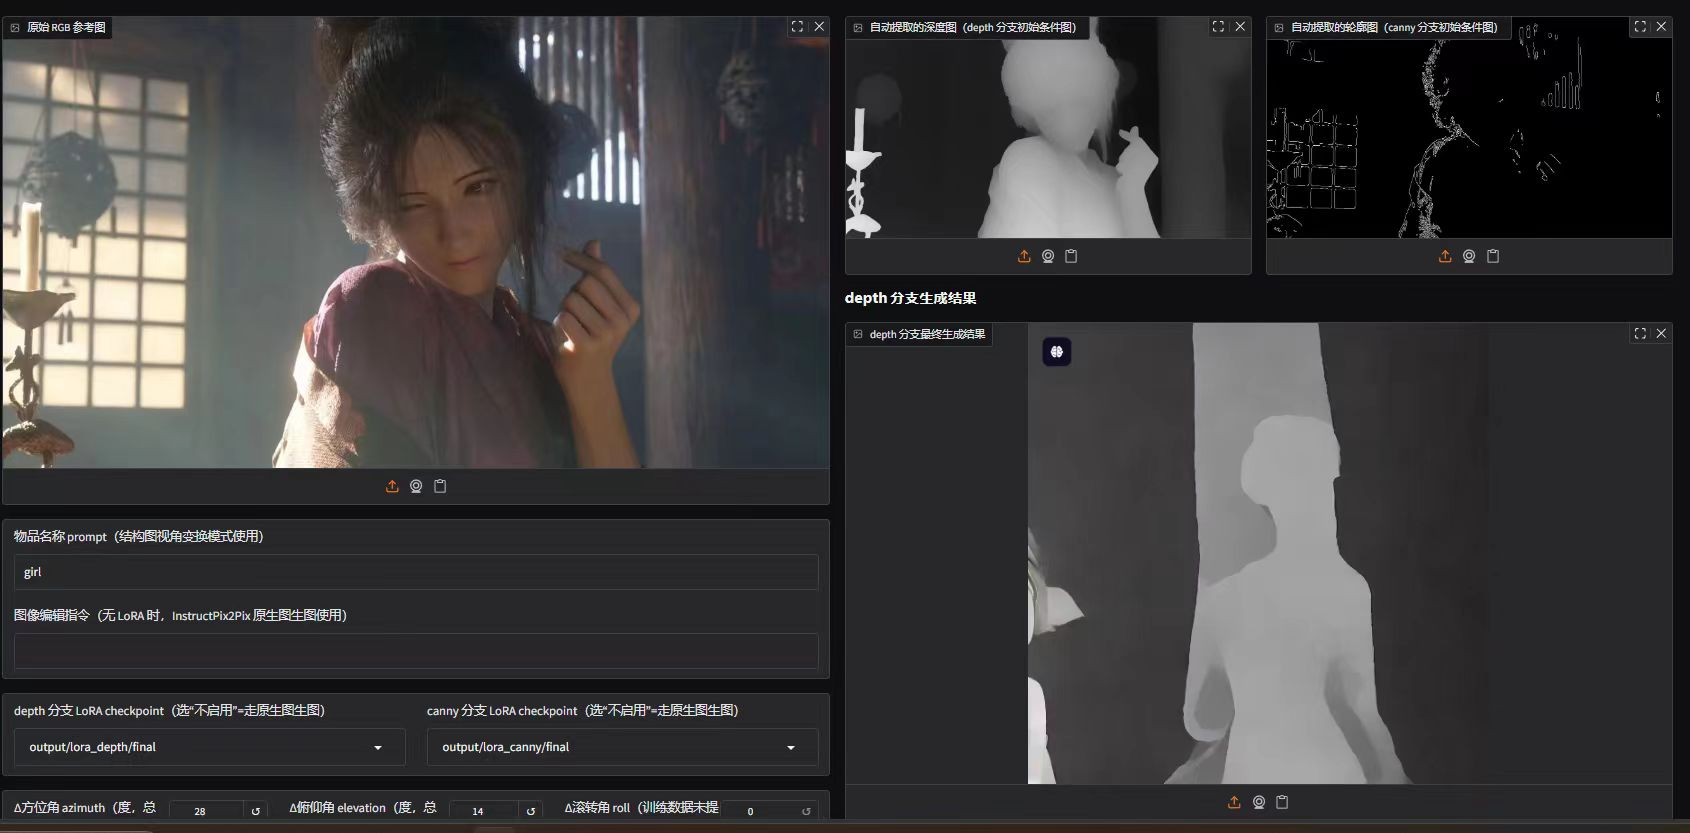
\includegraphics[width=\textwidth]{figures/gradio_ui.jpg}
    \caption{Gradio 推理调试界面。用户上传参考图后自动提取深度图与轮廓图，depth 与 canny 分支独立生成结果。}
    \label{fig:gradio_ui}
\end{figure}

\subsection{双模式推理}

InferencePipeline 类封装了两种互斥的推理模式，由 LoRA 目录是否为空自动切换：

\begin{itemize}
    \item \textbf{结构图视角变换模式}（LoRA 目录非空）：加载训练好的 LoRA + RotationEncoder 权重，走完整的"条件图 latent 拼接 + 旋转向量 cross-attention 注入 + 多步迭代"管线。
    \item \textbf{原生图生图模式}（LoRA 目录为空，默认）：直接调用 diffusers 官方的 \texttt{StableDiffusionInstructPix2PixPipeline}，以 InstructPix2Pix 底模原生的图像编辑能力对 RGB 参考图进行编辑。此模式不涉及 RotationEncoder 或条件 latent 拼接，但保证了"无 LoRA 时也能正常读图出图"，便于在 LoRA 训练完成前验证全链路。
\end{itemize}

\section{ComfyUI 工作流部署}

除了 Python 脚本推理外，项目还提供了 \texttt{camera\_control.json} ComfyUI 工作流，将核心流程封装为可视化节点图。工作流包含以下节点链：

\[
\text{Load Image} \to \text{Depth Anything V2} \to \text{ControlNet (Depth)} \to \text{KSampler} \to \text{VAE Decode} \to \text{Save Image}
\]

同时接入 Canny 边缘检测 + ControlNet (Canny) 并行路径，并加载 LoRA 权重。用户仅需替换输入图像与 prompt 即可运行，无需编写代码。运行硬件为 NVIDIA RTX 4060 16G，ComfyUI 工作流经过验证可稳定运行。

\section{运行环境与依赖}

训练与推理的 Python 依赖包括：PyTorch、Diffusers、Transformers、Accelerate、PEFT、Pillow、NumPy、OpenCV-Python 和 Gradio（完整列表见 \texttt{training/requirements.txt}）。数据集生成管线需要 Blender（可在命令行以 \texttt{--background} 模式调用）。所有实验在 Windows 系统、NVIDIA RTX 4060 16G GPU 上完成。
